%%%%%% CMB-S4 Simulations and Data Analysis Chapter, Time-Ordered Data Procesing Section  %%%%%%%%%%%%%%%%
 
\section{Time-Ordered Data Processing}

\subsection{Overview}

The time-ordered data processing elements of the CMB simulation and analysis pipeline -- simulation, pre-processing and mission characterization, and map-making -- are grouped as a subset due to the unique computational challenges posed by the volume of data that they must process.

\begin{figure}[htbp]
\centering
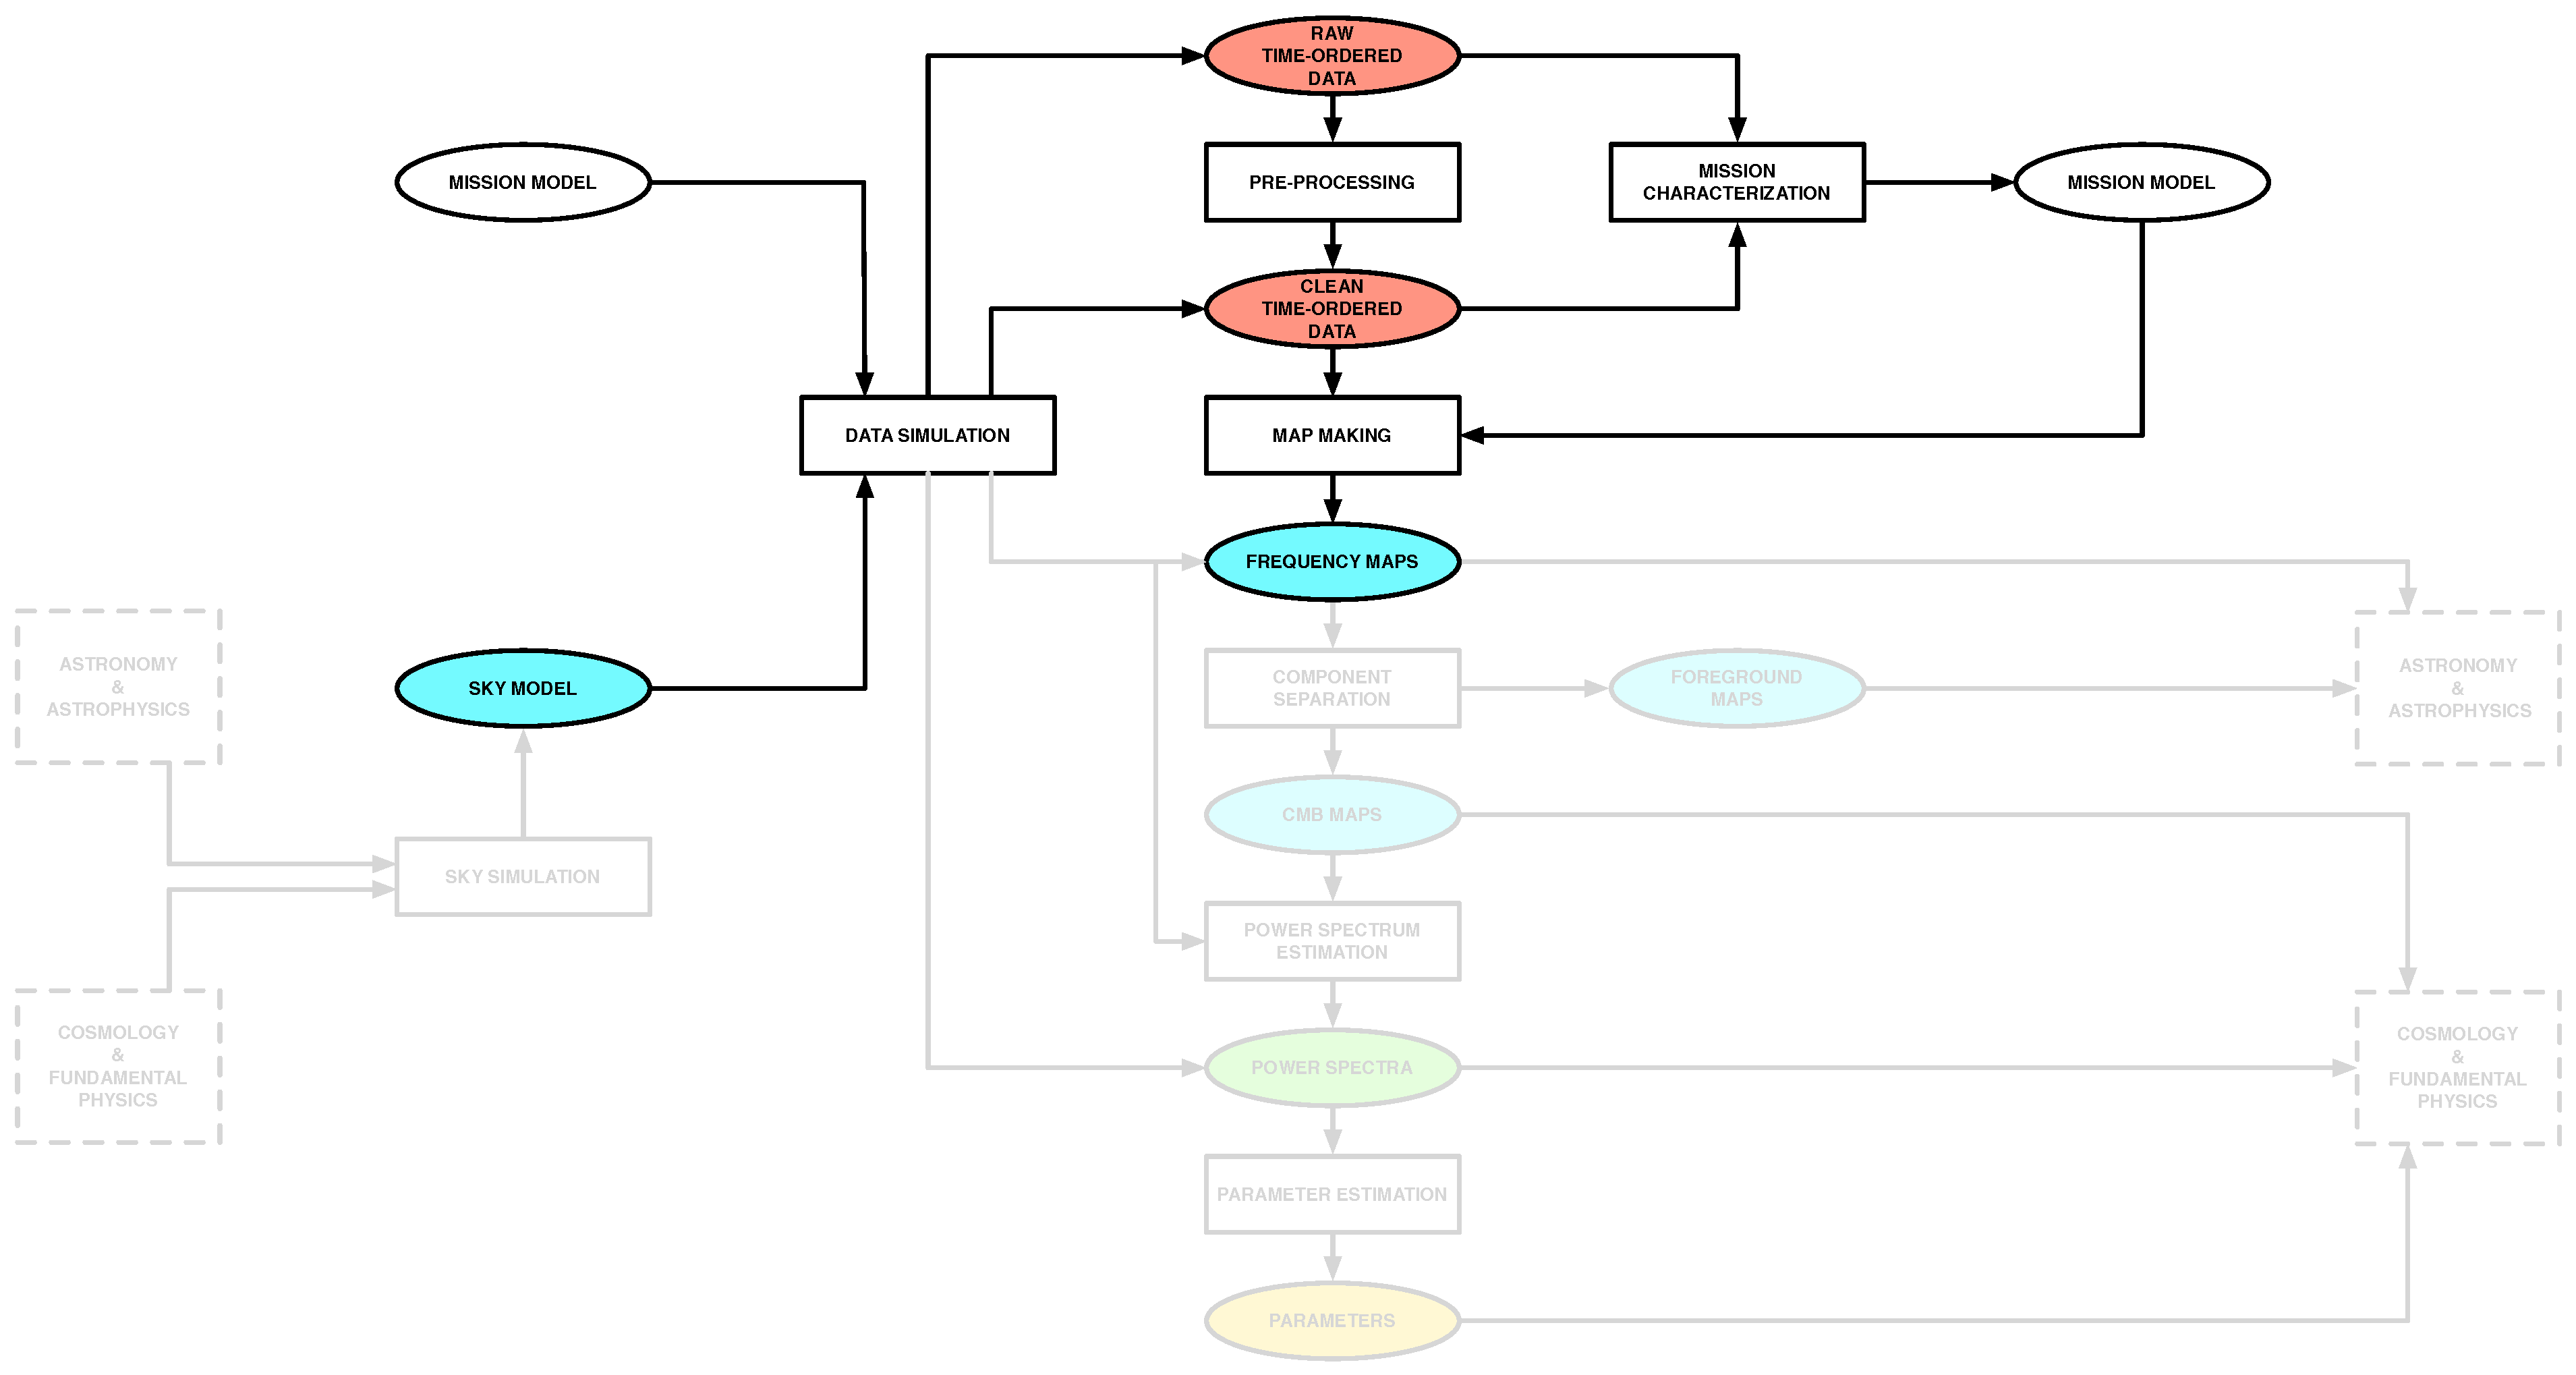
\includegraphics[width=1\textwidth]{Analysis/td}
\caption{The time-ordered data processing subset of the CMB simulation and data analysis pipeline}
\label{fig_td}
\end{figure}

\subsection{Simulation}

sky signal to instrument readout

instrument - beam, bandpass, noise; calibration, electronics

observation -- pointing, polarization (hwp), flagging, atmosphere

V \& V for other TOD processing elements

effective beam convolution

\subsection{Pre-Processing and Mission Characterization}

systematics mitigation: filtering, template-subtraction, marginalization

mission model building: pointing, beam, noise, systematics

\subsection{Map-Making}

Map-making is the stage of the analysis when the major compression of the time-ordered data happens and some estimate of the sky signal is produced at each observing frequency. It is usually a linear operation, characterized by some operator, $\mathbf{L}$, which transforms the input time-ordered data, $\mathbf{d}$, into a pixel domain map, $\mathbf{m}$, 
e.g., \cite{Tegmark1997},
\begin{eqnarray}
\mathbf{m} = \mathbf{L}\mathbf{d},
\end{eqnarray}
typically under the condition that the estimator is unbiased over the statistical ensemble of instrumental noise realizations, i.e.,
\begin{eqnarray}
\langle \mathbf{m} - \mathbf{s}\rangle = 0,
\label{eq:condMaps}
\end{eqnarray}
where $\mathbf{s}$ is the underlying pixelized sky signal. Given the usual model for the time-ordered data as the sum of sky-synchonous signal and time-varying noise, 
\begin{eqnarray}
\mathbf{d} = \mathbf{A}\mathbf{s} + \mathbf{n},
\end{eqnarray}
for a pointing matrix $\mathbf{A}$, this condition leads to,
\begin{eqnarray}
\langle \mathbf{m} - \mathbf{s}\rangle =  (\mathbf{L}\mathbf{A}-\mathbf{1})\mathbf{s} 
+ \langle \mathbf{n} \rangle = (\mathbf{L}\mathbf{A}-\mathbf{1})\mathbf{s},
\end{eqnarray}
as the average noise is assumed to vanish. Hence,
\begin{eqnarray}
\mathbf{L}\mathbf{A} = \mathbf{1},
\end{eqnarray}
which is solved by,
\begin{eqnarray}
\mathbf{L} = (\mathbf{A}^{\rm T} \mathbf{W} \mathbf{A})^{-1} \mathbf{A}^{\rm T} \mathbf{W}.
\end{eqnarray}
Here the matrix $\mathbf{W}$ is an arbitrary positive definite weight matrix, and different choices of $\mathbf{W}$ lead to different estimates of the sky signal.
\begin{itemize}
\item If $\mathbf{W}$ is taken to be the inverse of the time-domain noise covariance, i.e., $\mathbf{W} = \mathbf{N}^{-1}$, then the sky signal estimate, $\mathbf{m}$, will correspond to the {\bf maximum likelihood} and {\bf minimum variance} solution. 
\item If $\mathbf{W}$ is taken to be proportional to some diagonal matrix minus some low-rank correction, i.e. $\mathbf{W} \propto \mathbf{1} - \mathbf{T}\mathbf{T}^{\rm T}$,  with $\mathbf{T}$ assumed to be column-orthogonal, then the modes defined by its columns are marginalized over, effectively removing them from the solution. This approach includes as a special case so-called {\bf destriping} map-making, e.g.,~\cite{Poutanen2004, Keihanen2004}, which has gained recognition thanks to its successful applications to the Planck data, e.g.,~\cite{Keihanen2010, Tristram2011, LFIMaps2015, HFImaps2015}, and is therefore of potential interest to any experiments aiming to cover a large fraction of the sky. More generally, however $\mathbf{T}$ can be constructed to remove any unwanted modes present in the time domain data, e.g.,~\cite{Stompor2001, Cantalupo2010, Dunner2013}.
\item If $\mathbf{W}$ is taken to be diagonal, then the map-making solution corresponds to {\bf binning}, i.e. the weighted co-addition of the samples falling within each pixel.
\end{itemize}
If the instrument beams display complex, non-axially symmetric structure, the proper estimation of the sky signal may require correcting for their effects at the map level, leading to the so-called {\bf deconvolution} map-making ~\cite{ArmitageWandelt2004, Harrison2011, KeihanenReinecke2012}.  However, further work is needed to demonstrate the effectiveness of such an approach in general.

If map-making is used primarily as a data compression operation on the way to deriving constraints on the statistical properties of the sky signal (such as its power spectra), one may choose to relax the condition in Eq.~(\ref{eq:condMaps}) in favor of the more computationally tractable, albeit potentially biased, sky estimate,
\begin{eqnarray}
\mathbf{m} = (\mathbf{A}^{\rm T} {\rm diag}( \mathbf{W}) \mathbf{A})^{-1} \mathbf{A}^{\rm T}\mathbf{W} \mathbf{d},
\end{eqnarray}
where ${\rm diag}( \mathbf{W})$ denotes the diagonal part of $\mathbf{W}$. In this approach any bias is then corrected at the next level of the data processing, e.g.,~\cite{Hivon2002}. This approach has been proven to be very effective, at least in the context of experiments with small sky coverage, e.g., \cite{QUAD2010, SPT2011, POLARBEAR, BICEP2014}.

Formally the linearity of the mapmaking operation permits the propagation of the uncertainty due to the instrumental noise from time- to pixel-domain as
\begin{eqnarray}
{\hat{\mathbf{N}}} = \mathbf{L} \mathbf{N} \mathbf{L}^{\rm T},
\end{eqnarray}
which leads to a particularly simple expression for maximum likelihood estimators 
\begin{eqnarray}
{\hat{\mathbf{N}}} = (\mathbf{A}^{\rm T} \mathbf{N}^{-1} \mathbf{A})^{-1}.
\end{eqnarray}
However, as noted above, due its size the computational cost involved in computating such pixel-domain noise correlations make them impractical for all but special cases today, and the uncertainty is either carried over to the next stages of the data processing in implicit form or the final uncertainty is estimated using Monte Carlo simulations.

\subsection{Computational Constraints}



The computational requirements here are for both capacity and capability. To support the iterative exploration of the time-ordered data required by the pre-processing and mission characterization steps we need many analysts to be able to process the full data simultaneously, with each seeing no worse than order 1-day turnaround time for their jobs to complete. Conversely, to support the massive Monte Carlo simulation and map-making required for percent level uncertainty quantification in the absence of a full data covariance matrix, we need to be able to perform occasional runs of up to $10^4$ realizations within the total cycles available to us.

\begin{figure}[htbp]
\centering
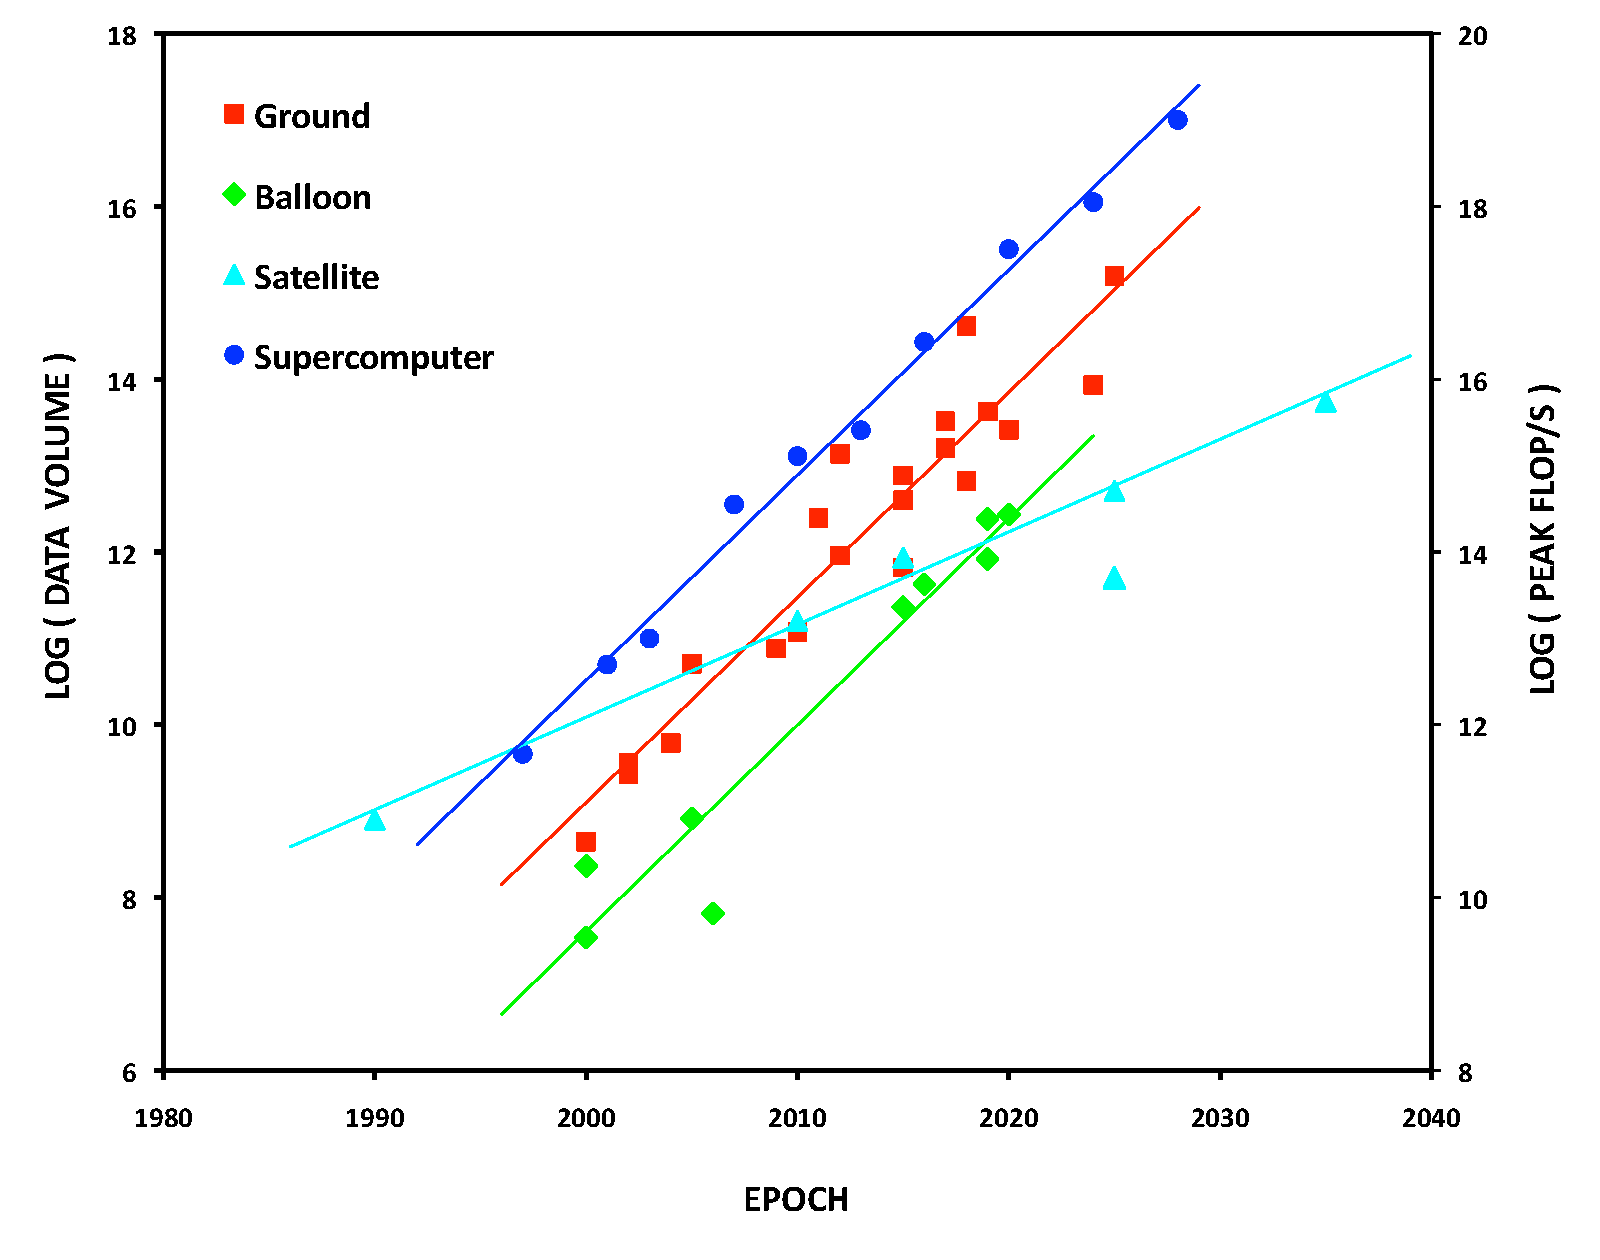
\includegraphics[width=0.5\textwidth]{Analysis/cmb_hpc_scaling}
\caption{Exponential growth of CMB time-ordered data volume and HPC capability: 1990 -- 2030.}
\label{fig_cmb_hpc_scaling}
\end{figure}

As Figure \ref{fig_cmb_hpc_scaling} shows, the size of ground-based, balloon-borne and satellite CMB data sets exhibit exponential growth over a 40 year period. Moreover, for suborbital experiments the exponent exactly matches that of Moore's Law, where we us as a proxy the peak performance of the flagship high performance computing (HPC) system at the DOE's National Energy Research Scientific Computing (NERSC) Center at any epoch (this choice reflecting the widespread use of NERSC for CMB data analyses over the last 20 years). 

As noted above, the intractability of pixel-domain data covariance matrices pushes us to use Monte Carlo (MC) methods for uncertainty quantification and debiasing, and the computational cost of the data analysis is dominated by the generation and reduction of sufficient MC realizations of the data for the resulting statistical error to be subdominant (typically assumed to be $10^4$ realizations for percent level uncertainty). 

Key challenges:
\begin{itemize}
\item computational tractability due to data volume and complexity of next-generation supercomputers
\item mitigating raw data systematics and developing sufficient mission and data models
\end{itemize}

All algorithmic and implementation choices we make must first and foremost be informed by their impact on computational tractability.

%\bibliography{cmbs4}

%%
%% Populate the .bib file with entries from SPIRES Bibtex (preferred)
%% or ADS Bibtex (if no SPIRES entry).
%%  SPIRES will also supply the CITATION line information; please include it.
%%


